\chapter{Deep Reinforcement Learning and Visual Servoing - A Literature Review}\label{chap: deep}
\section{Machine Learning}
In 1959 Arthur Samuel \cite{Puget} defined the concept of machine learning as \textit{"A field of study that gives computers the ability to learn without being explicitly programmed"}. The concept was further defined in 1998 when Tom Mitchell \cite{Puget} proposed a more precise definition as\\\\
\textit{"A computer program is said to learn from experience E with respect to some task T and some performance measure P, if its performance on T, as measured by P, improved with experience E"}\\\\
To clarify this definition we can look at an AUV performing a intervention task at a installation site. By doing this specific task, T, over and over again the performance measure, P, would be an indicator of how well the task is performed and the system will try to maximise this performance based on the experience, E.\\\\In the same way as machine learning can be viewed as a simple way of achieving Artificial Intelligence \cite{McClelland}, we achieve machine learning through three significant methods, see figure \ref{fig:ML}.
\begin{enumerate}
    \item Supervised Learning
    \item Unsupervised Learning
    \item Reinforcement Learning 
\end{enumerate}
\begin{figure}[H]
    \centering
    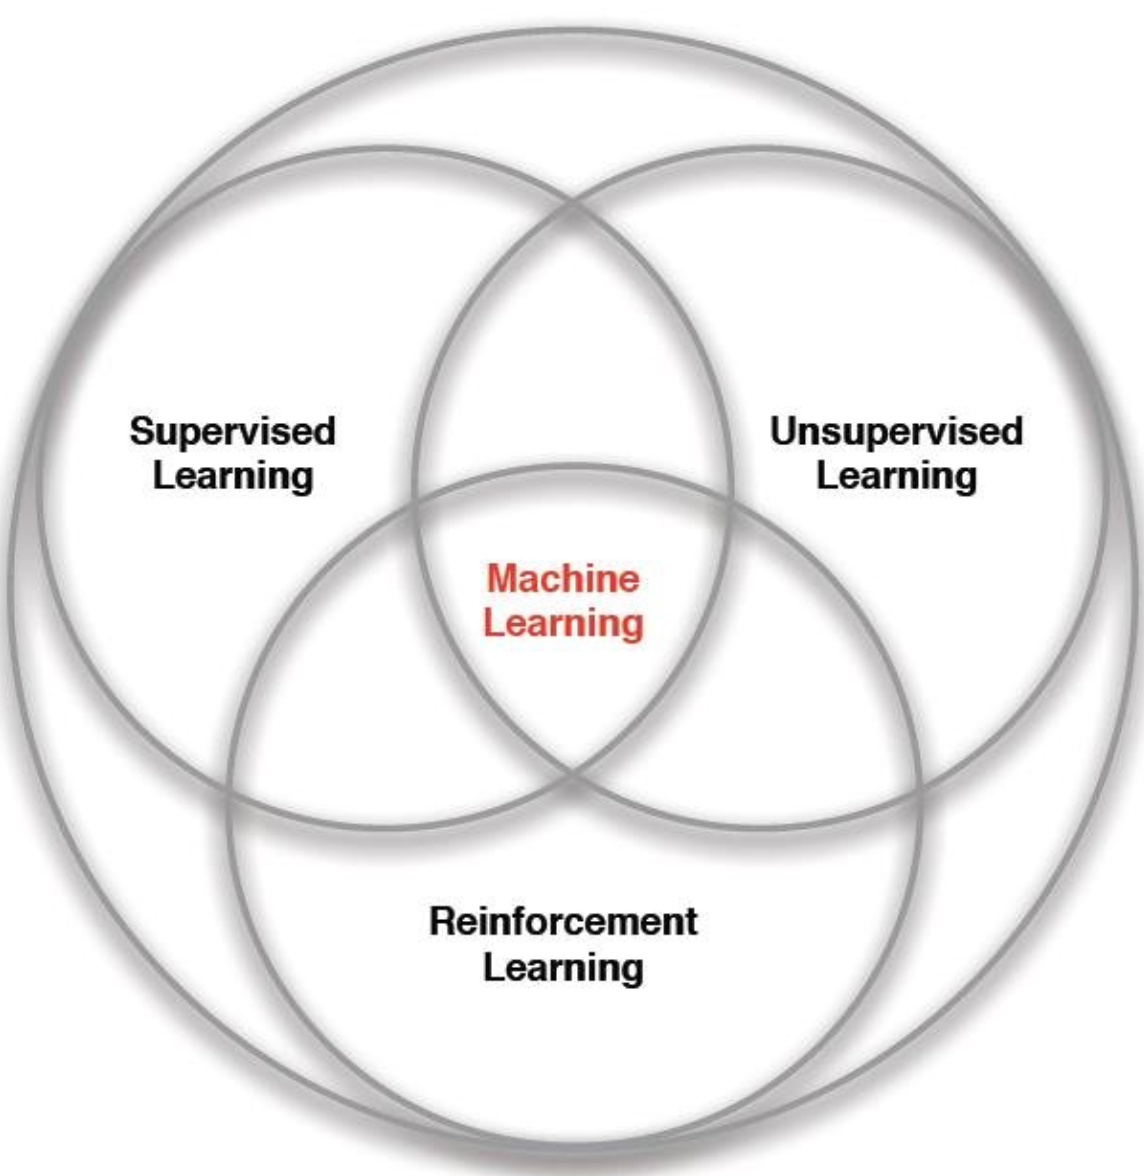
\includegraphics[width=0.5\textwidth]{images/chap2/ML.png}
    \caption{Machine Learning}
    \label{fig:ML}
\end{figure}
\textit{Supervised Learning} is the concept of using previous data to train an algorithm. By training the algorithm on large data-sets, preferable in the order of $10^{4}$ and larger, the goal is to learn the algorithm how to label any new data input. Defining this method in a mathematical sense the algorithm has access to both the input data, $X$, and the output data, $Y$, and tries to model-fit based on these. In example, we would use supervised learning for image classification by allowing the algorithm to train on a large data-set of images (\textit{input}) and labels (\textit{output}). If the algorithm is trained sufficient, the overall goal would be to use a new image as input, and have the algorithm output the correct label.\\\\
\textit{Unsupervised Learning}, on the other hand, is not given data to learn from, but the algorithm is left alone to discover interesting features in the data. Mathematically the algorithm has the input data, $X$, but no information about the output data. This branch of learning can be further divided into two sub-branches; \textit{Association} and \textit{Clustering}. In \textit{Association} the algorithm tries to discover "rules" which describes large portions of the data, in example "when the incident P occurs, L also tends to occur". In \textit{Clustering} the algorithm looks for clusters in the data, in example specific behaviour or trends. 

\section{An introduction to Reinforcement Learning}
In Reinforcement Learning the overall goal is to train an agent, in example an AUV, to perform correct actions in an environment. This is done by giving the agent a \textit{reward} based on how good it was to take a particular \textit{action} in the given state. The reward, $R_{t}$, is defined as a scalar feedback signal, indicating how good it was to take that action at that specific time-step, $t$. The overall goal is to maximise the total cumulative reward over all time-steps in order to find the optimal \textit{policy} to follow, starting in any state. By defining the reward as a scalar signal this means that we assume that every action in the real-world can be weighted against each other, meaning that even ethical dilemmas can be taken into account.\\\\
As stated, the goal of the Reinforcement Learning algorithm is to maximise the total cumulative reward. This is done by taking an action, $A_{t}$, in the environment. An important note her is that taking an action at the time-step $t$ might have a long-term consequence, meaning that the agent don't necessarily experience the consequence of taking that action in the next time-step. This is the same principle as i.e a financial investment.\\\\
In figure \ref{fig:environment} the relationship within Reinforcement Learning is visualised. For each time-step, $t$, the agent will execute an action, $A_{t}$, receive an observation, $O_{t}$ and a scalar reward, $R_{t}$. The environment will receive an action, $A_{t}$, and return an observation, $O_{t}$ and a scalar reward, $R_{t}$ to the agent. 
\begin{figure}[H]
    \centering
    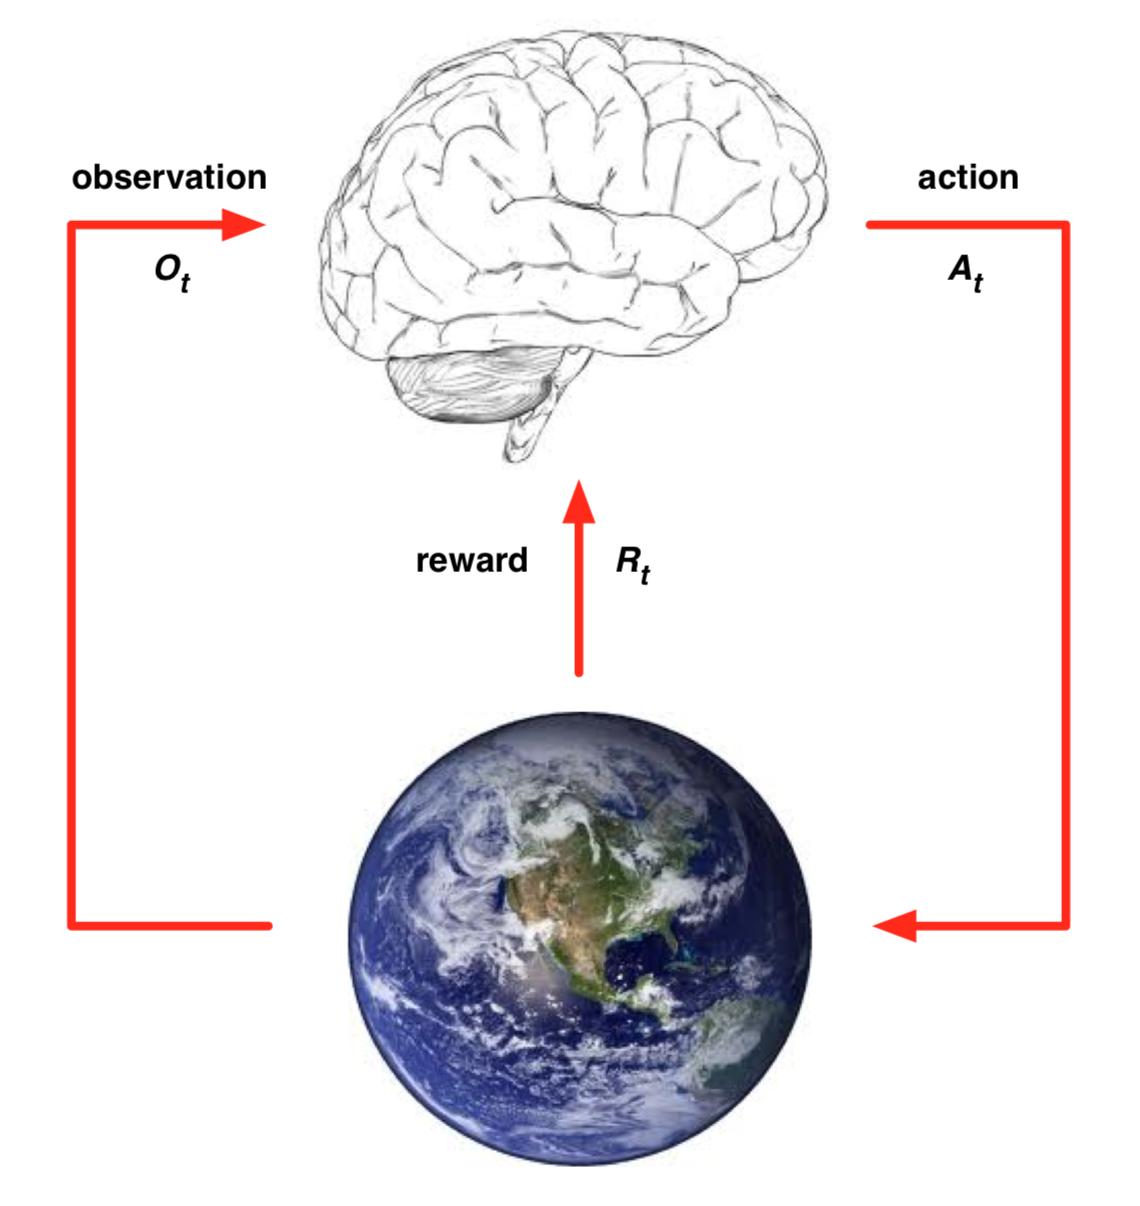
\includegraphics[width=0.5\textwidth]{images/chap2/Agent_environment.png}
    \caption{Reinforced learning environment \cite{Silver}}
    \label{fig:environment}
\end{figure}
\subsection{Markov Decision Processes}
When introducing the concepts of Reinforcement Learning it is necessary to determine what types of \textit{environments} that are possible to "solve" using this technique. A \textit{Markov Decision Process} (MDP) describes a fully $observable$ environment for Reinforcement Learning. A given state, $S_{t}$, is said to be $Markov$ if and only if
\begin{equation}
    P[S_{t+1}] = P[S_{t+1} | S_{1},...,S_{t}]
\end{equation}
In all generality the $\textit{Markov Property}$ states that \textit{the future is independent of the past given the present}, meaning that the state will capture all the relevant information from the history, but the history may be erased once the state is known.\\\\
In an environment where all states are Markov, a \textit{Markov Decision Process} is a Markov reward process with decision. This is given by a tuple $$<\mathcal{S, A, P, R, \gamma}>$$Where
\begin{itemize}
    \item $\mathcal{S}$ - a finite set of states.
    \item $\mathcal{A}$ - a finite set of actions.
    \item $\mathcal{P}$ - a state transition probability matrix.
    \item $\mathcal{R}$ - a reward function, where $\mathcal{R}^{a}_{s} = \mathbb{E}[R_{t+1}|S_{t}=s, A_{t} = a]$.
    \item $\mathcal{\gamma}$ - a discount factor, $\gamma \in [0, 1]$.
\end{itemize}
The reason for using a discount factor, $\mathcal{\gamma}$, has several advantages. From a mathematical prospective it is convenient to discount, as well as making sure that infinite returns are avoided. Furthermore, there is also an uncertainty about the future that is unknown, and the agent do not know if an immediate reward is more valuable than a future reward. In \textit{Markov Decision Processes} three definitions are essential; the \textbf{policy}, $\pi$, the \textbf{state-value} function, $V_{\pi}(s)$, and the \textbf{action-value} function, $q_{\pi}(s,a)$. 
\begin{itemize}
    \item The \textit{policy}, $\pi$, determines how the agent behaves in the environment, meaning which policy it is following. The policy is dependent on the current state, $S_{t}$, and the action taken, $A_{t}$, in that state. This is defined as
    \begin{equation}
        \pi(a|s) = \mathbb{P}[A_{t}=a | S_{t} = s]
    \end{equation}
    \item The \textit{state-value function}, $V_{\pi}(s)$, is the expected return, $G$, by starting in a state, $s_{t}$, and following a specific policy, $\pi$. The state-value function is defined as 
    \begin{equation}
        V_{\pi}(s) = \mathbb{E}_{\pi}[G_{t}|S_{t}=s]
    \end{equation}
    \item The \textit{action-value function}, $q_{\pi}(s,a)$, takes the action into account. Computing the expected return, $G$, by starting in a state, $s_{t}$, taking an action, $a_{t}$, and following a policy, $\pi$. The action-value function is defined as
    \begin{equation}
        q_{\pi}(s,a) = \mathbb{E}_{\pi}[G_{t}|S_{t}=s, A_{t} = a]
    \end{equation}
\end{itemize}
These three definitions are the essential for optimising the MDP. In order to use them the \textit{Bellman Expectation Equation} \cite{Silver} is introduced, which transforms the
definitions above into a new set of \textbf{solvable} definitions. This means that both the state-value function and the action-value function can be decomposed into an immediate reward plus the discounted value of the successor state. This is given as
\begin{itemize}
    \item \textit{Bellman Expectation Equation} for the state-value function, $V_{\pi}(s)$, is given by
    \begin{align}
        V_{\pi}(s) & = \mathbb{E}_{\pi}[R_{t+1}+\gamma V_{\pi}(S_{t+1})|S_{t}=s] \\
        & = \sum_{a\in \mathcal{A}} \pi(a|s)(\mathcal{R}_{s}^{a}+\gamma \sum_{s'\in \mathcal{S}} \mathcal{P}_{ss'}^{a} V_{\pi}(s'))
    \label{eq:bell1}
    \end{align}
    \item \textit{Bellman Expectation Equation} for the action-value function, $q_{\pi}(s,a)$, is given by
    \begin{align}
        q_{\pi}(s,a) & = \mathbb{E}_{\pi}[R_{t+1}+\gamma q_{\pi}(S_{t+1}, A_{t+1}) | S_{t} = s, A_{t} = a] \\
        & = \mathcal{R}_{s}^{a}+\gamma \sum_{s'\in \mathcal{S}} \mathcal{P}_{ss'}^{a} \sum_{a' \in \mathcal{A}} \pi(a'|s')q_{\pi}(s',a')
    \label{eq:bell2}
    \end{align}
\end{itemize}
By doing this the algorithm is able to look one step ahead based on the current state and the action policy it is following. This concept can be explained through a \textit{Look-ahead tree}, which is illustrated in figure \ref{fig:lookahead}. Overall, this look-ahead tree lets the agent evaluate how "\textit{good}" it is to take a particular action given the current state. 
\begin{figure}[H]
    \centering
    \begin{subfigure}[b]{0.45\textwidth}
        \centering
        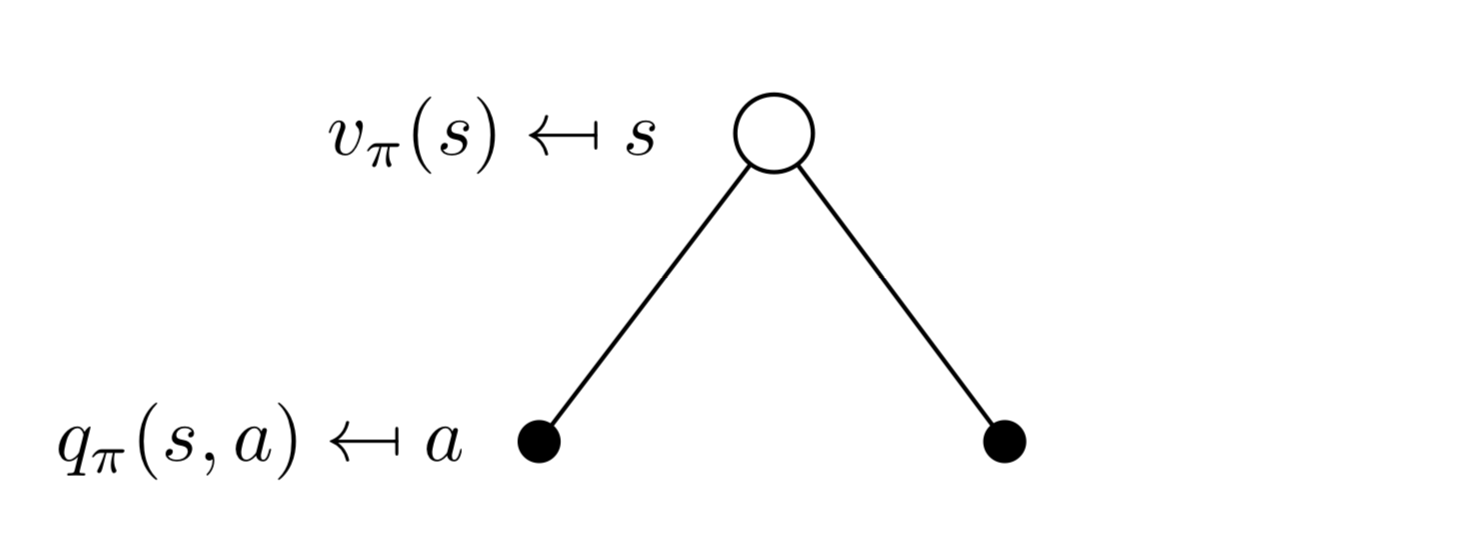
\includegraphics[width=\textwidth]{images/chap2/look-ahead-value.png}
        \caption{state-value function}
    \end{subfigure}
    \hfill
    \begin{subfigure}[b]{0.45\textwidth}
        \centering
        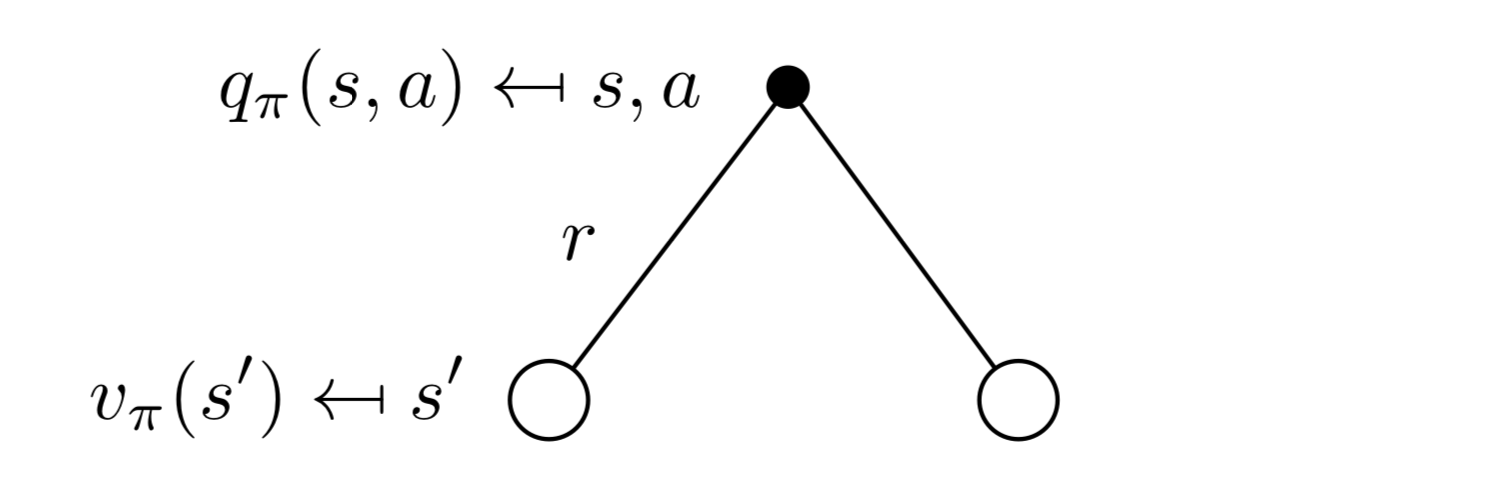
\includegraphics[width=\textwidth]{images/chap2/look-ahead-action-value.png}
        \caption{action-value function}
    \end{subfigure}
    \caption{Look-ahead tree\cite{Silver}}
    \label{fig:lookahead}
\end{figure}
The overall goal of the MDP is to find the optimal behaviour for the agent, this means that the MDP is "solved" when the agent has found the optimal value function, meaning the best possible policy. This is done by taking the maximum value function, $max_{\pi}$, over both the state-value function and the action-value function. The optimal policy for the agent can then be found by maximising over the optimal action-value function. In conclusion, MDPs, which are environments consisting of a tuple $$<\mathcal{S, A, P, R, \gamma}>$$, is therefore very suitable to solve with Reinforcement Learning. The tuple above also shows that an underwater environment can be defined as an MDP. The state, $S$, would be the location of the AUV in the environment, the action, $A$, would be the direction the AUV is taking in the given state, and the reward, $R$, would say something about how good it is for the AUV to go in this specific direction, based on the objective. By defining the underwater environment as an MDP it shows that Reinforcement Learning can be applied to \textit{solve} control problems in the underwater environment.
\subsection{Dynamic Programming}
Solving MDPs often results in a complex and computational costly process, this is where \textit{Dynamic Programming} comes in handy. Dynamic Programming is a method for solving complex problems, where the problem is broken down into sub-problems, and solved separately, before combining the solutions \cite{Silver}. Dynamic Programming works very well for problems with the following properties; \textit{Optimal substructure}, meaning that the problem can be decomposed into $overlapping$ $sub-problems$, resulting in solutions that can be cached and reused. In MDPs, using the Bellman equation results in a recursive decomposition, with the value function both storing and reusing solutions, which means that MDPs satisfies both properties.\\\\
In Reinforcement Learning the dynamic programming algorithm will take the MDP, $<\mathcal{S, A, P, R, \gamma}>$, as input, and return the optimal value function, $V_{*}$, and an optimal policy, $\pi_{*}$. The way it does this is by iterative apply the Bellman Expectation Equations from equation \ref{eq:bell1} and \ref{eq:bell2}. This is done by starting of with an arbitrary initial value function, and sweep over all states in each iteration. The policy is improved by acting $greedily$ with respect to $V_{\pi}$, given by $\pi'=greedy(V_{\pi})$. This concept is illustrated in figure \ref{fig:greedily}. The algorithm initialises an arbitrary state-value and policy function, then it evaluate these, and act greedily to receive an improved state-value and policy function. By iterative doing this the policy will \textbf{always} converge to the optimal value-function, $V^{*}$, and the optimal policy, $\pi^{*}$. 
\begin{figure}[H]
    \centering
    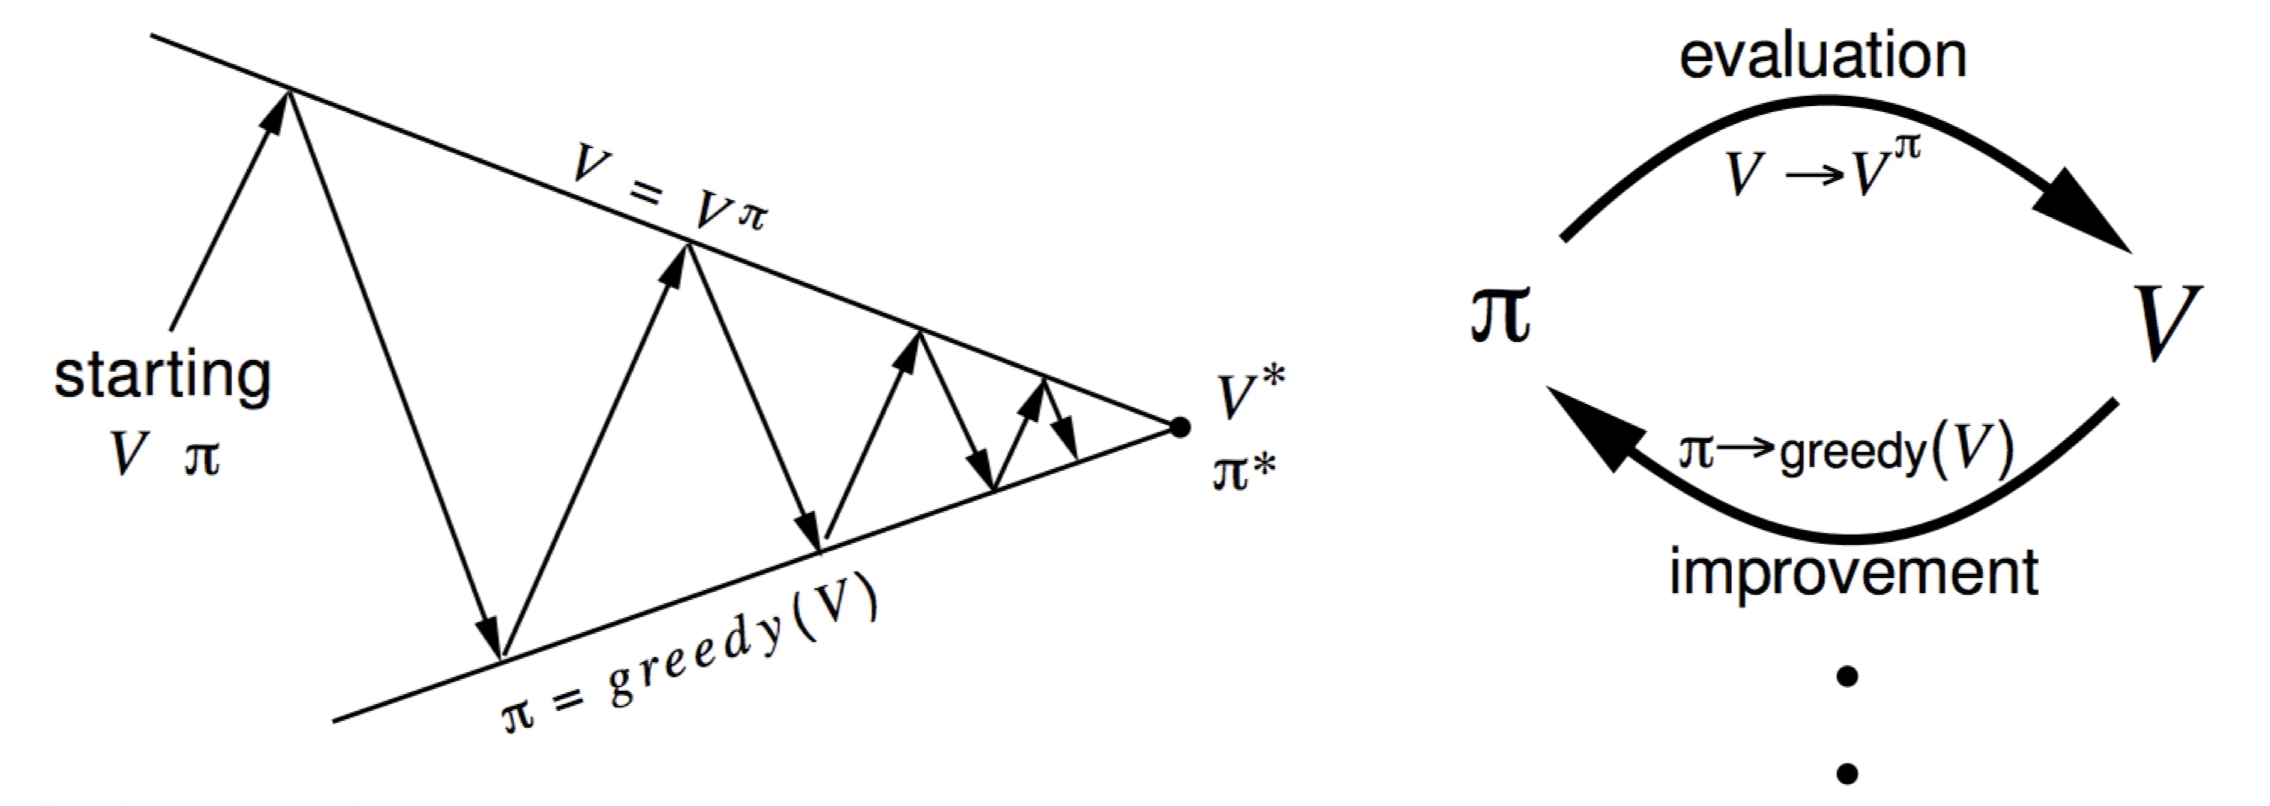
\includegraphics[width=0.75\linewidth]{images/chap2/policy-iteration.png}
    \caption{Policy iteration by acting greedily\cite{Silver}}
    \label{fig:greedily}
\end{figure}

\section{Visual servoing}
The purpose of \textit{Visual servoing} techniques is to control a dynamic system, such as an AUV, by extracting information from a vision sensor \cite{Quentin}. Through the use of multiple cameras the agent is able to extract detailed information about the environment, in the same way as humans. Classical approaches of visual servoing are based on extracting, tracking and matching a set of visual features; points, lines or moments, which are used to move the unit towards a desired pose by using them as input in a control law. \\\\
Extracting, tracking and matching these visual features are a complex task, much because of the high-fidelity information from cameras. In \cite{Collewet} Photometric visual servoing, a method with no feature extraction requirements, was introduced as a possible solution to resolve the complexity of the task. However, compared to classical approaches this solution has a very small convergence domain because of the high non-linearity's between the 3D unit motion and image information. Other, more optimistic, solutions to the problem have centred around using \textit{neural networks}. Deep neural networks, especially \textit{Convolutional Neural Networks} (CNN), have during the recent years contributed to a great leap in a number of computer vision tasks, including: image classification \cite{Hinton}, depth map prediction \cite{Eigen} and real-time 6-DOF camera relocalization \cite{Kendall}. In order to get a better understanding of how the neural networks can be used in robotics it is reasonable to discover how these convolutional networks operates. 
\subsection{Convolutional Neural Networks}
\textbf{Artificial Neural Networks} (ANNs) are based on the idea of how biological nervous systems, such as the human brain, operates \cite{Keiron}. The basic idea of ANNs are to process neurons, interconnected computational nodes, to learn from the input in order to optimise the output. In figure \ref{fig:ann} a common ANN architecture is illustrated, with an \textit{input layer}, a \textit{hidden layer} and an \textit{output layer}. Here the input layer, which usually takes in a multi-dimensional vector, will distribute to the hidden layers, which will make decisions based on the previous layer and see how this improves or detriments the output. This is called the process of learning, and by having multiple hidden layers we commonly refer to it as \textit{deep learning} \cite{McClelland}.
\begin{figure}
    \centering
    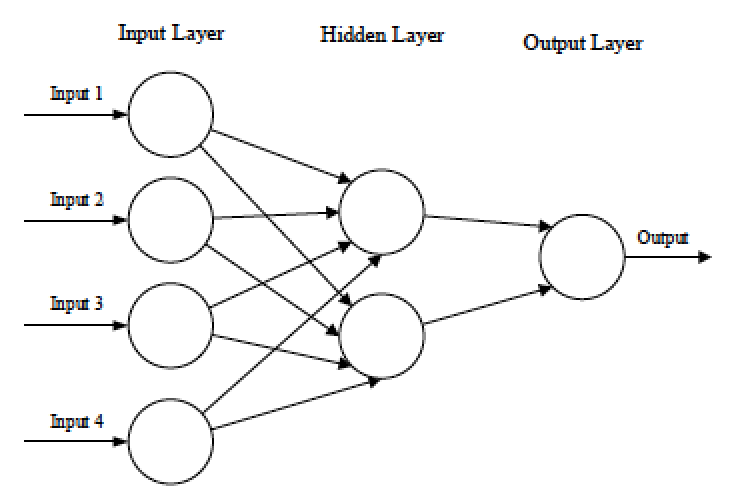
\includegraphics[width=0.7\textwidth]{images/chap2/ANN.png}
    \caption{Common ANN architecture }
    \label{fig:ann}
\end{figure}
\textbf{Convolutional Neural Networks} (CNNs) is based on the same principles of using neurons that self-optimise through learning, as traditional ANNs. As in ANNs each neuron receives an input and perform a operation, and the journey from the raw image vectors to the final score is still being expressed as a single perceptive score function, while the last layer contains loss functions in relation to the classes.\\\\
CNNs differs from ANNs in the way that they are mainly used within pattern recognition in images. The advantage of using these is that they allows us to encode features specific for the image into the architecture, which makes the network better for image-specific tasks.  
\subsubsection{CNN architecture}
In figure \ref{fig:cnn} a simple overview of the relevant components in CNN architecture is visualised. In general the CNN architecture can be divided into three types of layers
\begin{enumerate}
    \item The \textbf{convolutional layer} will apply a convolution operation, which reduces the number of free parameters, to the input, and sends the results to the next layer. The reason for applying the ReLu (\textbf{rectified linear unit}) layer in figure \ref{fig:cnn} is to apply an element-wise activation function to the output from the previous layer. 
    \item The \textbf{pooling layer} continues to reduce the number of parameters, by performing down-sampling along the spatial dimensional of the input from the convolutional layer. 
    \item The \textbf{fully-connected layers} completes the process by attempting to construct class scores from the activations, in order to classify the output. 
\end{enumerate}
\begin{figure}[H]
    \centering
    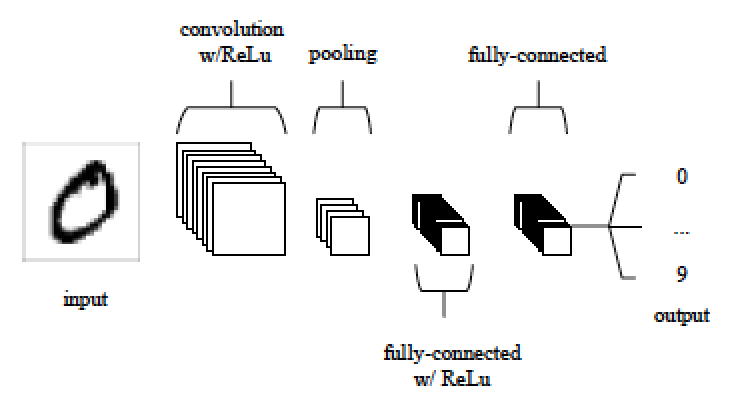
\includegraphics[width=0.7\linewidth]{images/chap2/CNN.png}
    \caption{CNN architecture \cite{Keiron}}
    \label{fig:cnn}
\end{figure}
The overall advantage of having this architecture when applying CNN to image classification problems is that any image can be defined on a \textit{matrix form}, making the layers defined above very intuitive to use. 
\subsubsection{Convolutional layer}
The \textbf{convolutional layer}, which is visualised in figure \ref{fig:convolutional}, aims to detect specific features in the image input, by the use of learnable \textbf{kernels}, which are filters with spatial dimensionality that spreads along the entire image input. Each kernel will produce a 2D activation map when the input makes impact with the layer, and the scalar product is then calculated for each kernel value. The weights of the kernel determines what specific feature that is detected, and our network therefore learns the specific feature based on which kernels that are "firing" activation maps. The kernels that "fires" are defined as \textbf{activations}, and the activation map from each kernel will be placed along the entire depth dimension of the input, to make the full output volume from the layer.
\begin{figure}[H]
    \centering
    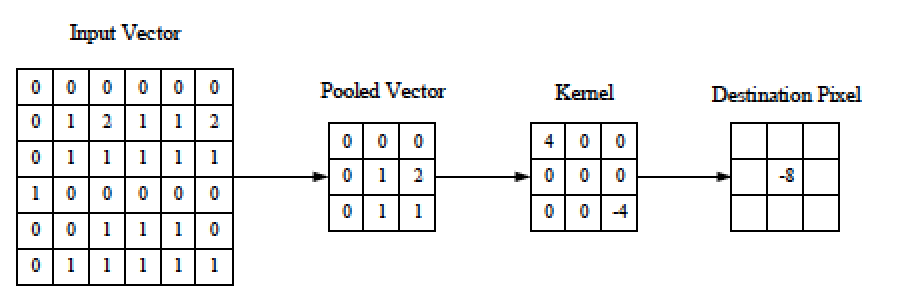
\includegraphics[width=0.7\textwidth]{images/chap2/convolutional_layer.png}
    \caption{Convolutional layer architecture \cite{Keiron}}
    \label{fig:convolutional}
\end{figure}
As shown in figure \ref{fig:convolutional} the centre element of the kernel matrix is placed over the input vector, which then calculates the scalar product and is replaced by a weighted sum based on the neighbour pixels. In the beginning of the section it was stated that ANNs are ineffective on image recognition because of the data size, and thereby the computational power needed to train effectively. The reason for this was that ANN neurons are defined in a fully-connected manner. To resolve this the convolutional layer in CNNs are only connected to a \textit{small} volume of the input, and the dimension of this volume is usually referred to as the \textbf{receptive field size} of the neuron. To see how this resolves the computational complexity we can look at an 64 x 64 x 3 input image, which is an \textit{RBG} image with dimension of 64 x 64. If the receptive field size is set as 6 x 6 this would result in $6*6*3=108$ weights on each neuron, but if we used the same input with standard ANNs it would contain $64*64*3=12,1288$ weights.\\\\
The convolutional layers uses three optimisation hyper-parameters in order to reduce the complexity of the output; \textbf{depth}, \textbf{strides} and \textbf{zero-padding}.
\begin{itemize}
    \item The \textbf{depth} of the output is manually set based on the number of neurons within the layer, by reducing this parameter we can minimise the total number of neurons in the network and reduce complexity of the output. However, there is a trade-off in doing this, since less neurons also results in reduced pattern recognition capabilities.
    \item The \textbf{stride} of the output, which is the depth surrounding the spatial dimensionality that places the receptive field, can also be set manually. In example, by choosing this equal to 1 it would produce large activations, because we have heavily overlapping receptive fields. Increasing the stride will however reduce the overlapping and result in lower spatial dimensions.
    \item The \textbf{zero-padding} means "padding" the input border, which gives us further control of the output volume dimension.
\end{itemize}
All these optimisation parameters will impact the spatial dimensionality of the output from the convolutional network. The impact can be calculated by
\begin{equation}
    \frac{(V-R)+2Z}{S+1}
\label{eq:spatial}
\end{equation}
where V is the input volume, R is the receptive field size, Z the amount of zero-padding and S is the stride \cite{Keiron}. The output of equation \ref{eq:spatial} needs to be equal to an integer. If this is not the case the stride has been defined wrong, meaning that the neurons will not be able to fit smoothly across the input. 
\subsubsection{Pooling layer}
The output from the convolutional layer will be sent further on to the \textbf{pooling layer}. The pooling layer will further reduce the dimension of the input through reducing the computational complexity and the number of parameters.\\\\
This is done through the use of a \textbf{max} function, which usually is defined with kernels of dimension 2 x 2 and a stride of 2 along the spatial dimension of the input. Overall, the use of a pooling layer will reduce the activation map with $\approx$ 75 percent of the original size, while still maintaining the depth of the input volume. This reduction can be seen in figure \ref{fig:convolutional}. 
\subsubsection{Fully-connected layers}
Finally the \textbf{fully-connected layer} is attached at the end of the network. In all simplicity this layer will take in an input volume from the convolutional layer, ReLu or the pooling layer, and output a vector specifying the number of detection classes the program can choose from, i.e cat, dog, etc. 


